% Docker Meetup at MfN, 24 April 2018
% Running wikis at the Museum with Docker - past, present and future
% Alvaro Ortiz-Troncoso
% 
% Template:
% see https://en.wikibooks.org/wiki/LaTeX/Presentations

\documentclass[13pt]{beamer}
\usepackage[utf8]{inputenc}
\usepackage{graphicx}
\usepackage{xcolor}

\definecolor{mfn_green}{HTML}{A1BF23}
\setbeamercolor{title}{fg=black}
\setbeamerfont{title}{family=\sffamily,series=\bf}
\setbeamercolor{frametitle}{fg=black}
\setbeamerfont{subtitle}{family=\sffamily,shape=\itshape}
\beamertemplatenavigationsymbolsempty
\setbeamertemplate{footline}[page number]
\setbeamertemplate{itemize item}{\color{mfn_green}$\blacktriangleright$}
\setbeamertemplate{caption}{\tiny \insertcaption}
\setbeamersize{text margin left=5mm,text margin right=5mm}

% Running wikis at the Museum with Docker: past, present and future The Museum outputs exhibitions, science papers, conferences, and so much more. None of this would be possible without cooperation between researchers, designers, organizers and of course admins and developers. Wikis were introduced at the Museum in 2014 as an %experiment to improve  cooperation within project teams. I'll talk about how Docker solves many of the problems of running a bunch of wikis on a string, and also about pending questions we are currently trying to answer. I am a computer scientist and joined the Museum in 2014. I have worked at the Technische Universität Berlin and at Waag Technology & Society in Amsterdam.

\title
{Running wikis at the Museum with Docker}
\subtitle{past, present and future}
\author
{Alvaro Ortiz-Troncoso}
\date
{Docker Meetup at Museum für Naturkunde Berlin, 2018}
\subject{Computer Science}

\begin{document}

% 1. Titelseite
{
  \logo{
\includegraphics[height=1cm]{mfn_logo_klein.png}\vspace{220pt}}
  \frame{\titlepage}
}

% 2. Das Museum
% This talk is about our experience with combining Docker and wikis at the Museum. First I'll talk shortly about what we do at the Museum, and how we do it. The Museum is a very dynamic environment, and working here is probably very different from what most people imagine. Then I'll talk about running wikis with Docker. I'll go into the reasons for adopting Docker, both organisational and technical. Finally, I'll talk about plans for the future. Particularly regarding our plans, I'm very interested in hearing your feedback, criticism, and ideas.  
\begin{frame}
  \frametitle{Das Museum / \textcolor{mfn_green}{The Museum}}
  \begin{figure}
    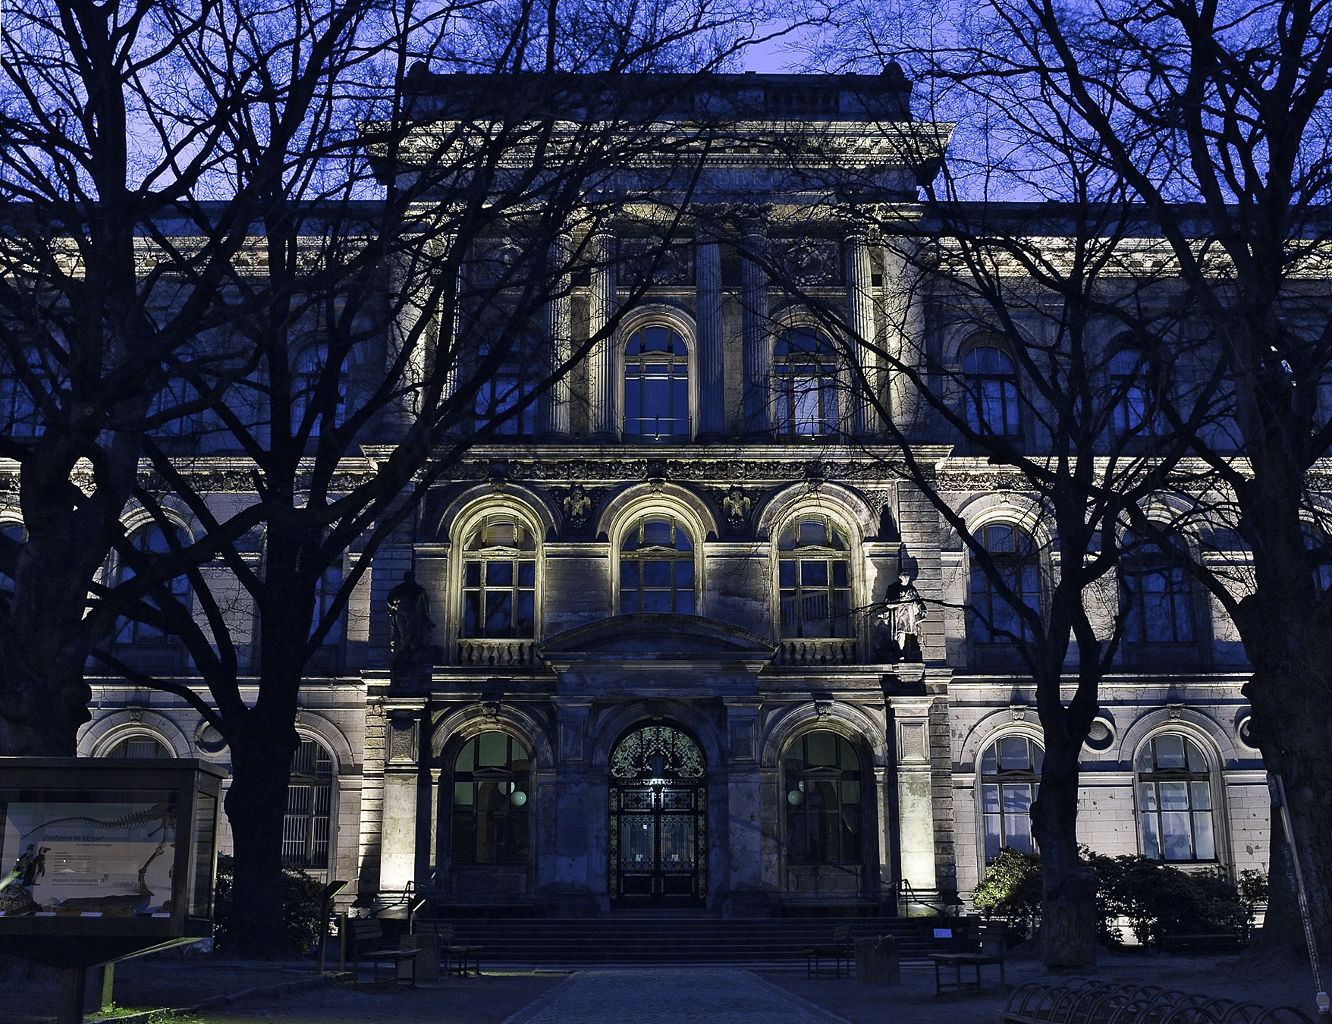
\includegraphics[height=70mm]{Gebaeude_Nacht.jpg}
    \caption{\textcopyright Antje Dittmann, Museum für Naturkunde Berlin, 2009. CC-by-sa}
  \end{figure}
\end{frame}

% 3. Ausstellung
% Most people think the Museum is the exhibition. This is partly true, but there is much more going on behind the scenes Of course, many people know that museums cannot display everything they have. But most people are unaware of the amount of research that is carried out on the collection.
\begin{frame}
  \frametitle{Die Ausstellung / \textcolor{mfn_green}{The exhibition}}
  \begin{figure}
  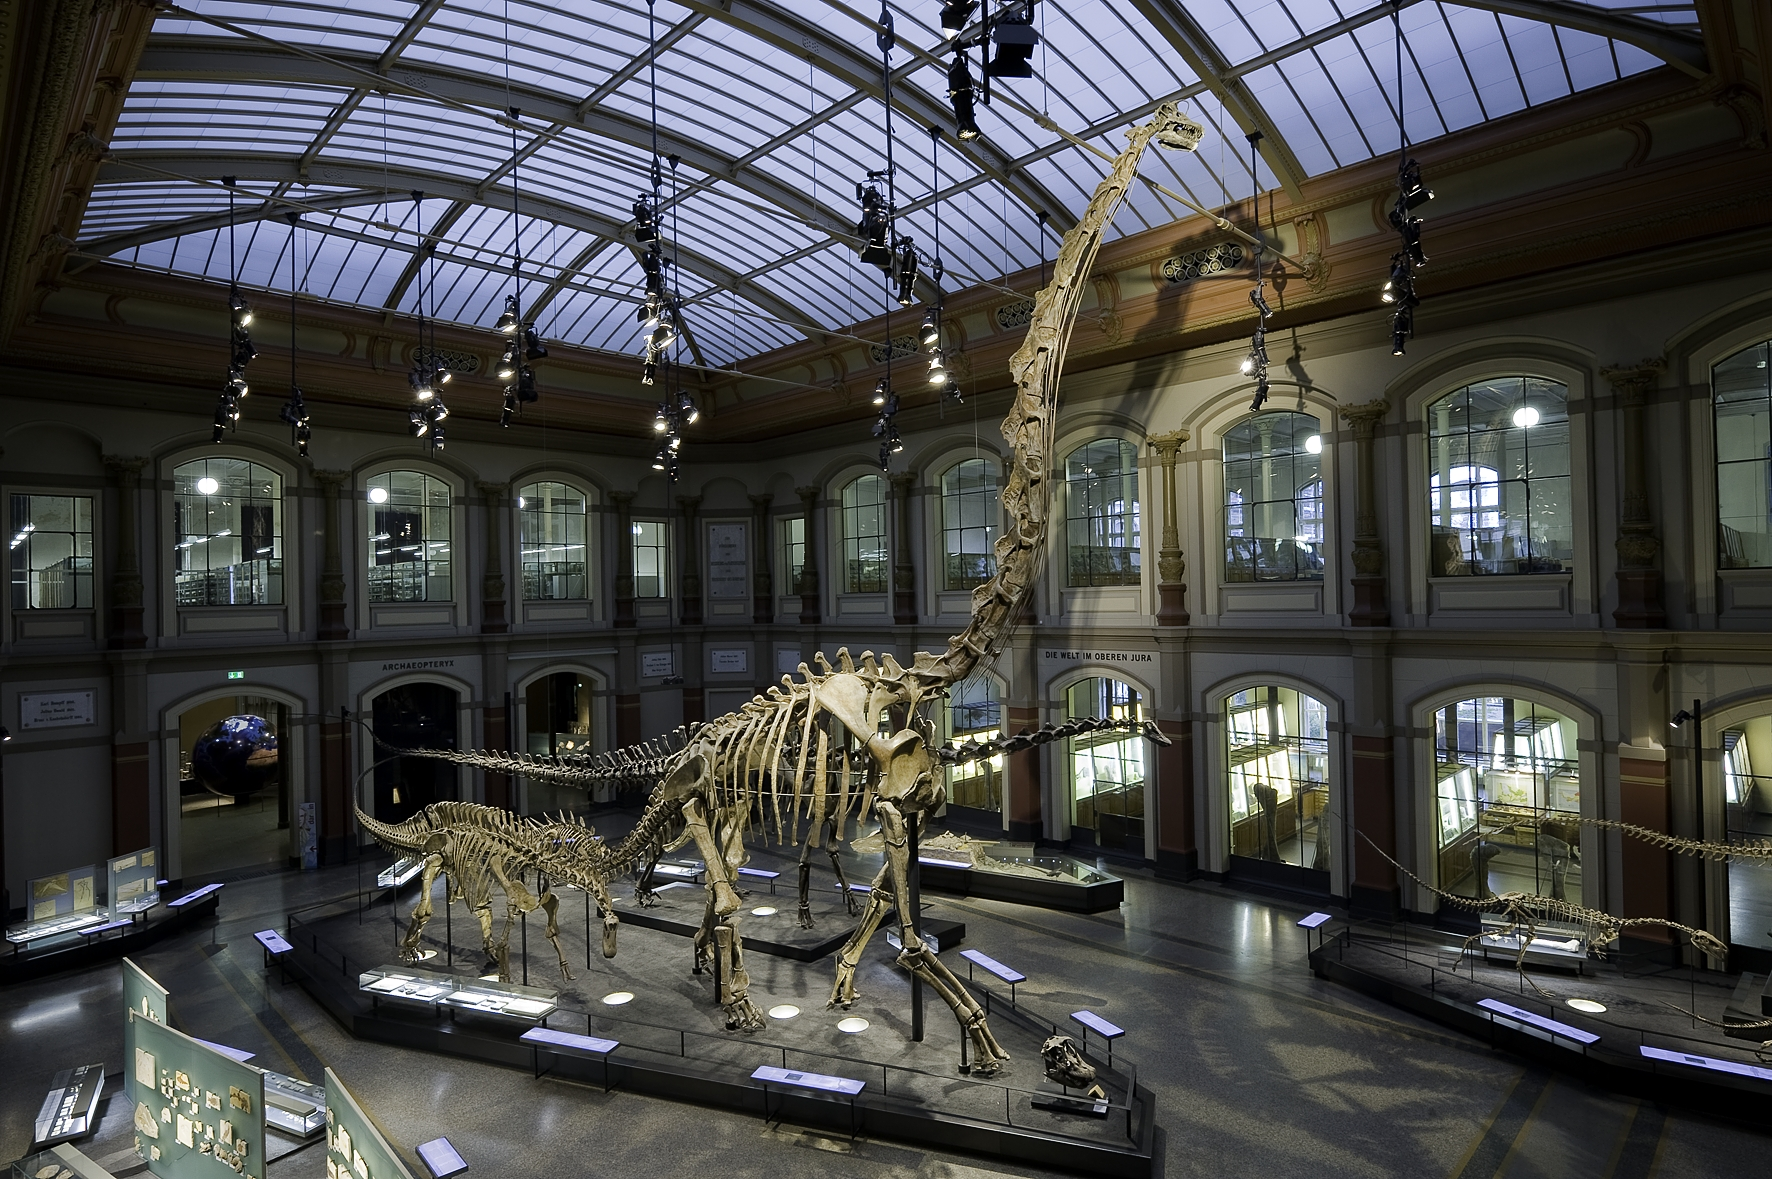
\includegraphics[height=70mm]{Brachiosaurus_02_15cm.jpg}
  \caption{\textcopyright Antje Dittmann, Museum für Naturkunde Berlin, 2009. CC-by-sa}
  \end{figure}
\end{frame}

% 4. Einige Zahlen
% Almost 500 persons work at the museum, including scientists, students, lab technicians, software developers and so on. As in any science institution, output can be measured by the number of publications. These include science publications but also books and articles in magazines. There are currently 51 research projects actively working on the collection.
\begin{frame}
  \frametitle{ Einige Zahlen / \textcolor{mfn_green}{Some numbers}}

  \begin{itemize}
  \item{Personal: 289, Studenten: 209}
  \item{Publikationen: 222 / Jahr (2016)}
  \item{Aktuell erforschen 51 Projekte die Sammlung}
  \end{itemize}
  
  \begin{itemize}
  \item{\textcolor{mfn_green}{Staff: 289, Students: 209}}
  \item{\textcolor{mfn_green}{Publications 222 / year (2016)}}
  \item{\textcolor{mfn_green}{Currently 51 projects are researching the collection}}
  \end{itemize}
  \bigskip
  \begin{center}\tiny{Unsere Wissenschaft / Our Science, DOI: 10.7479/3dwq-8a7g}\end{center}
\end{frame}

% 5. Forschungsprojekte
% Here are some examples of research projects: the Museum hosts a number of laboratories, where research is carried out in many fields, such as genetics. The Museum is using 3D-scanners to digitise the collection. The Museum is also involved in ecological projects, for example in mapping the biological diversity in certain regions, for example in Indonesia. Geologists at the Museum are modelling planetary impacts, and meteorites. The Museum also developed an App, that can be downloaded from the App-Store, that helps to identify birds by song and plants using a mobile phone. There are just a few almost randomly chose examples of projects. There are many more, they are presented on the Museum website if you are interested.
\begin{frame}
  \frametitle{Forschungsprojekte / \textcolor{mfn_green}{Research projects}}
  \begin{figure}
  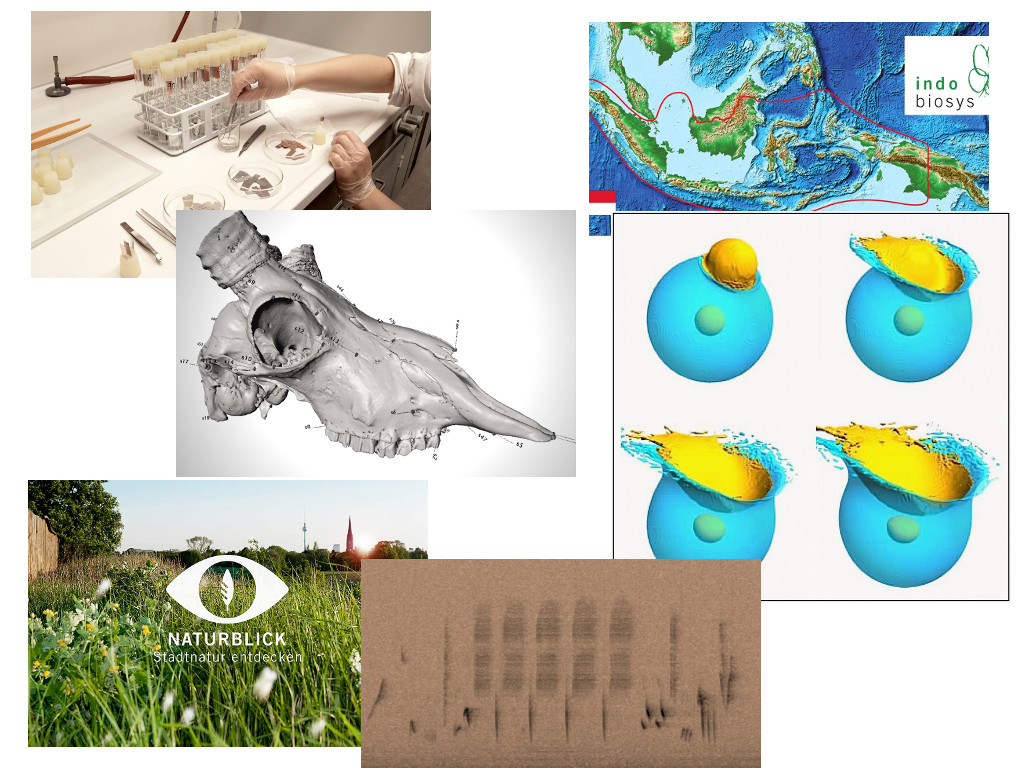
\includegraphics[height=70mm]{Forschung.jpg}
  \caption{https://www.museumfuernaturkunde.berlin/}
  \end{figure}
\end{frame}

% 6. Was macht ein Projekt aus?
% On the one hand, the Museum is meant to preserve and curate the collection, forever. On the other hand, we do all this exhiting, dynamic stuff. This is possible because research projects are set up in a very similar way to projects in a start-up. A project basically needs 3 things: funding, a time plan (a project has a beginning and an end), and most importantly a team. Research teams at the Museum often include a researcher and collaborators from many different fields, such a software developers, system administrators, management people, designers or photographers, lab technicians and so on.
{
\setbeamercolor{background canvas}{bg=mfn_green}
\setbeamercolor{frametitle}{fg=black}
\begin{frame}
  \frametitle{Was macht ein Projekt aus? \\ \textcolor{white}{What does it take to launch a project?}}
  \begin{figure}
  \includegraphics[height=70mm,trim=4 4 4 4,clip]{Projekt.png}
  \end{figure}
  \bigskip
\end{frame}
}

% 7. Kooperation
% Cooperation is necessary for at least 3 reasons: a team that is made of persons coming from different fields and specialities, needs to come to a common understanding of what it is they wish to achieve. For example, "success" for a scientist might be something totally different than "success" for a manager. So achieving a common understanding of project goals is necessary. Cooperation is also necessary to deliver on time. As anybody who has worked on a project can tell, there is never enough time. Cooperation is also necessary to work efficiently and deliver within budget.
\begin{frame}
  \frametitle{Kooperation / \textcolor{mfn_green}{Cooperation}}

  \begin{itemize}
  \item{Gemeinsames Verständnis der Projektziele}
  \item{Innerhalb des Zeitrahmens zum Ergebnis kommen}
  \item{Den Kostenrahmen nicht überschreiten - Effizient arbeiten}
  \end{itemize}
  
  \begin{itemize}
  \item{\textcolor{mfn_green}{Common understanding of project goals}}
  \item{\textcolor{mfn_green}{Deliver on time}}
  \item{\textcolor{mfn_green}{Be efficient to finish within budget}}
  \end{itemize}
\end{frame}

%%%%%%%%%%%%%%%
%
% The past
%
%%%%%%%%%%%%%%%

% 8. In der Vergangenheit
\begin{frame}
  \frametitle{In der Vergangenheit / \textcolor{mfn_green}{In the past}}
  \begin{figure}
    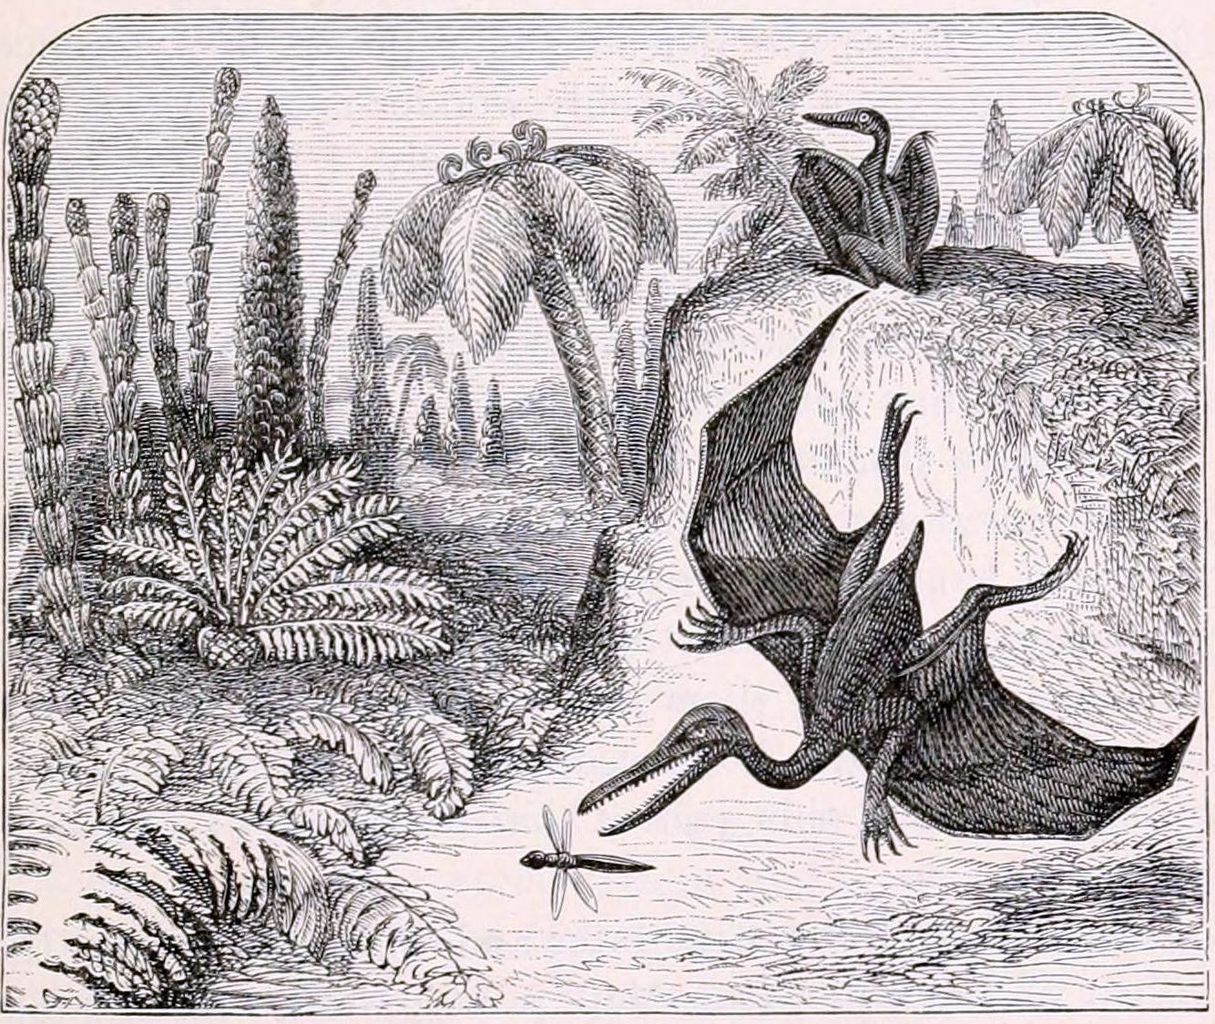
\includegraphics[height=70mm]{Ideal_Landscape_of_a_Prehistoric_Age.jpg}
    \caption{Quackenbos, J.D., 1886. \textit{Illustrated School History of the World}. D. Appleton.}
  \end{figure}
\end{frame}

% 9. Word .doc Hölle
% In the past, the only way to cooperate was through exchanging paper documents. Unfortunately, many people still think this way, except that Word documents have replaced paper. So a primitive way of cooperating is to place a Word document on a shared drive and to email the documents address to your collaborators. As Word does not support collaboration, this means that a document that is opened for editing by one person cannot be edited by anyone else. As this happens very often, people have taken to sending documents as email attachments, which is a definitive receipt for final chaos. 
{
\setbeamercolor{background canvas}{bg=mfn_green}
\setbeamercolor{frametitle}{fg=black}
\begin{frame}
  \frametitle{Word\textsuperscript{\tiny\textregistered} .doc Hölle /
    \textcolor{white}{Word\textsuperscript{\tiny\textregistered} .doc hell}}
  \begin{figure}
  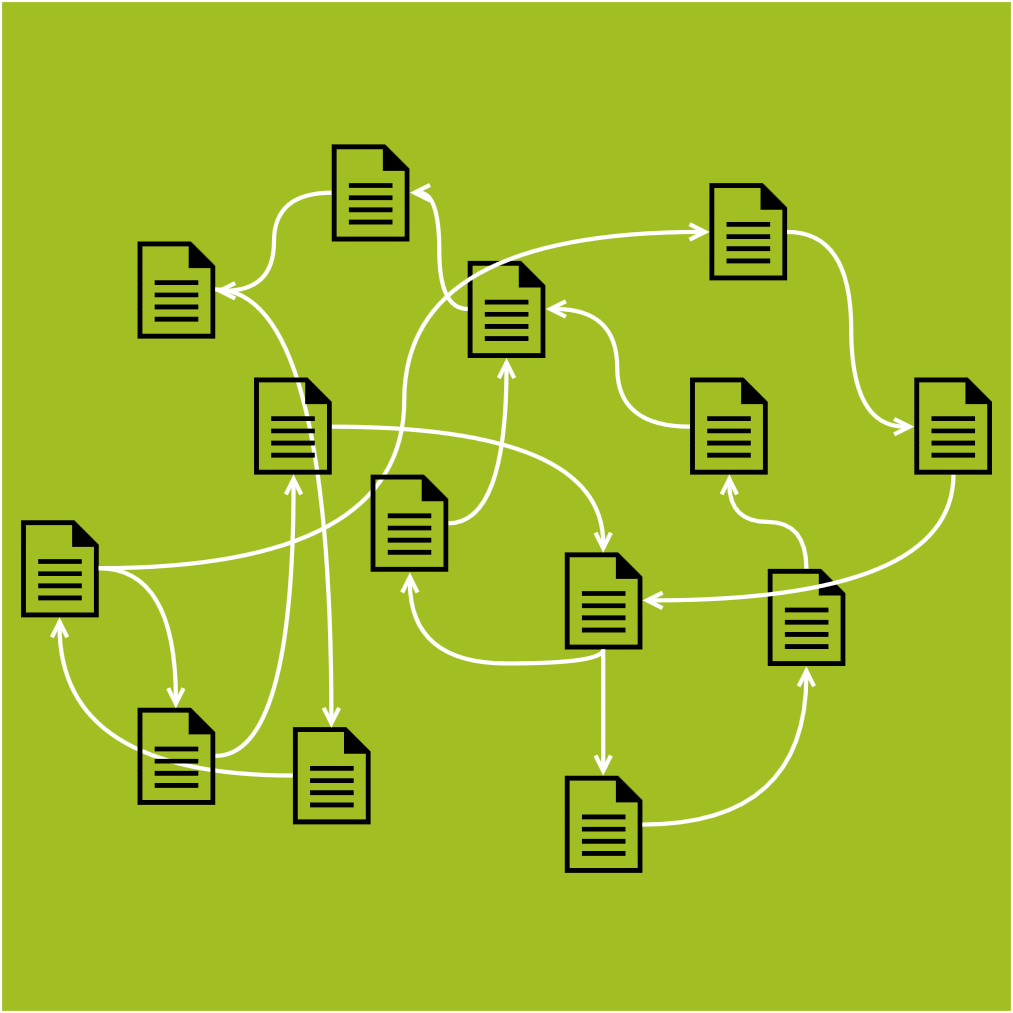
\includegraphics[height=70mm,trim=4 4 4 4,clip]{Docs.png}
  \end{figure}
\end{frame}
}

% 10. Nichts gegen Word aber...
% Although Word is quite a good programme, when it comes to collaboration it has some very clear disadvantages: There is no way to know which one of the document copies is the final version, or if there are several versions, there is no way to automatically merge documents. Word does not provide a transparent mechanism to follow who wrote which part of a document. Authorship is very important for researchers, as researchers build up their scientific reputation by publishing. Another important drawback of Word is that it is a proprietary format. The Museum has been around since 1889 and will survive not only all of us, but very probably also Microsoft, and what happens then?
\begin{frame}
  \frametitle{Nichts gegen Word\textsuperscript{\tiny\textregistered} aber... \\
    \textcolor{mfn_green}{Absolutely nothing against Word\textsuperscript{\tiny\textregistered}, however, ...}}
  \begin{itemize}
  \item{Keine Versionierung: wer hat die Endfassung?}
  \item{Kein Dokumentverlauf: wer hat was geschrieben?}
  \item{Proprietäre Software: Anbieterabhängigkeit}
  \end{itemize}
  
  \begin{itemize}
  \item{\textcolor{mfn_green}{No versioning: who has the final version}}
  \item{\textcolor{mfn_green}{No document history: who wrote what?}}
  \item{\textcolor{mfn_green}{Proprietary software: vendor lock-in}}
  \end{itemize}
\end{frame}

%%%%%%%%%%%%%%
%
% The present
%
%%%%%%%%%%%%%%

% 11 Beispiel Panda-Wiki
% For these reasons, the Museum decided to set up a collaboration environment. When I joined the Museum in 2014, my first job was to experiment with wikis to create such an environment. There are currently 24 wikis at the Museum, here is an example: the wiki of the Panda exhibition. This wiki is interesting because it went through the life-cycle of a whole project: during project planing, it was used to write texts for the labels in the exhibition, and to gather material for the exhibition catalogue. During the exhibition, it was made public and was used as exhibition website. After the exhibition, the wiki can now be used as exhibition archive.
\begin{frame}
  \frametitle{Konkretes Beispiel: das Panda-Wiki\\\textcolor{mfn_green}{A specific example: the Panda wiki}}
  \begin{figure}
    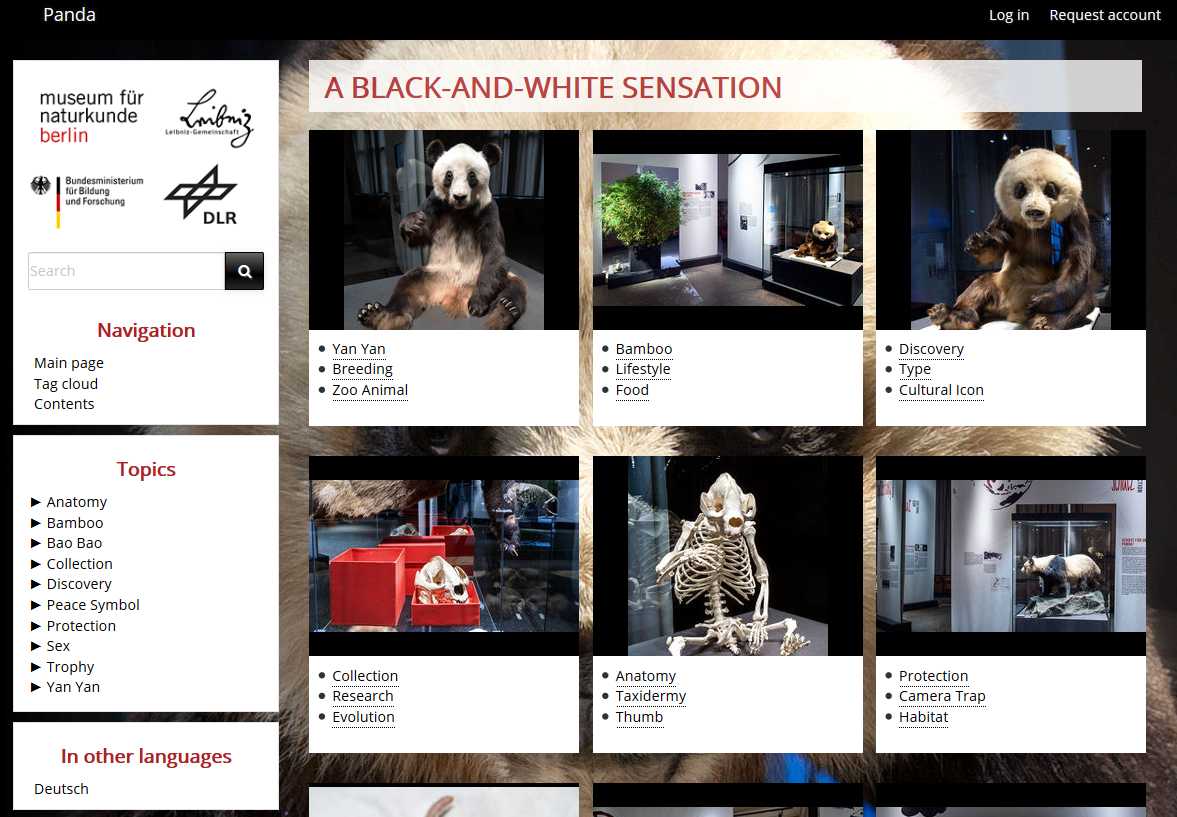
\includegraphics[height=60mm]{panda.png}
    \caption{http://biowikifarm.net/v-mfn/panda}
  \end{figure}
\end{frame}

% 12. Wikis am Museum
% Research projects at the Museum may use a wiki to support collaboration within a team, if they wish to do so. Although projects at the Museum can be of very different kinds, the wikis have some requirements in common. Two important requirements are: wikis are by default private. Scientists are sometimes reluctant to share their data and results before their research has been published, as scientists are specially rewarded for publishing unheard-off results. These are the rules of the game in academia. The second important requirement is that wikis should be semantic. This means that our wikis are capable of storing free-form texts, in a similar way than Wikipedia can deal with texts, but can also store structured data. Information in the wiki can then be queried in various ways, and that increases value of the information stored in the wiki. 
\begin{frame}
  \frametitle{Wikis am Museum / \textcolor{mfn_green}{Wikis at the Museum}}

  \begin{itemize}
  \item{Forschungsprojekte können ein Wiki nutzen, sofern sie es wünschen}
  \item{Wikis sind standardmäßig privat, können aber zum Teil oder im Ganzen geöffnet werden}
  \item{Wikis sind semantisch: sie können sowohl mit Freiformtexten als auch mit strukturierten Daten umgehen}
  \end{itemize}
  
  \begin{itemize}
  \item{\textcolor{mfn_green}{Research projects may use a wiki if they wish to do so}}
  \item{\textcolor{mfn_green}{Wikis are private by default, but may be made public in part or in whole}}
  \item{\textcolor{mfn_green}{Wikis are semantic, so can be used with plain texts as well as with structured data}}
  \end{itemize}
\end{frame}

% 13. Die derzeitige Praxis
% In a nutshell, running projects requires collaboration. Collaboration has to be supported by a collaboration environment. Setting up a collaboration environment requires software infrastructure and processes. I'll go into more detail on the steps of this process on the next slide, and also into the problems this process has. Doing things this way has a very important advantage: a clear separation of concerns and responsibilities between the system administrators and the developers. System administrators are Museum staff, and they can concentrate on building the Museum's infrastructure, which is what they do best. Developers are temporary project staff or external contractors, and the can concentrate on pushing their project forward.
\begin{frame}
  \frametitle{Die derzeitige Praxis / \textcolor{mfn_green}{The current practice}}
  \begin{figure}
    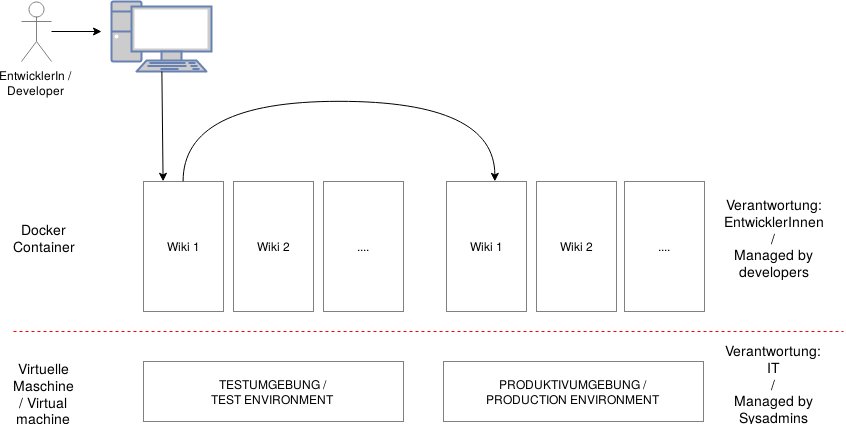
\includegraphics[width=110mm]{docker_wikis.png}
  \end{figure}
\end{frame}

% 14. Rolloutprozess
% A detailed look at the roll-out process, as it is implemented now. The current practice at the Museum is that new wikis are first build as a Docker image by a developer, at the developers desktop computer. Then the Docker images are uploaded to a test server for testing. If they pass the tests, the images are deployed to the production server.
\begin{frame}
  \frametitle{Rolloutprozess / \textcolor{mfn_green}{Roll-out process}}

  \begin{figure}
    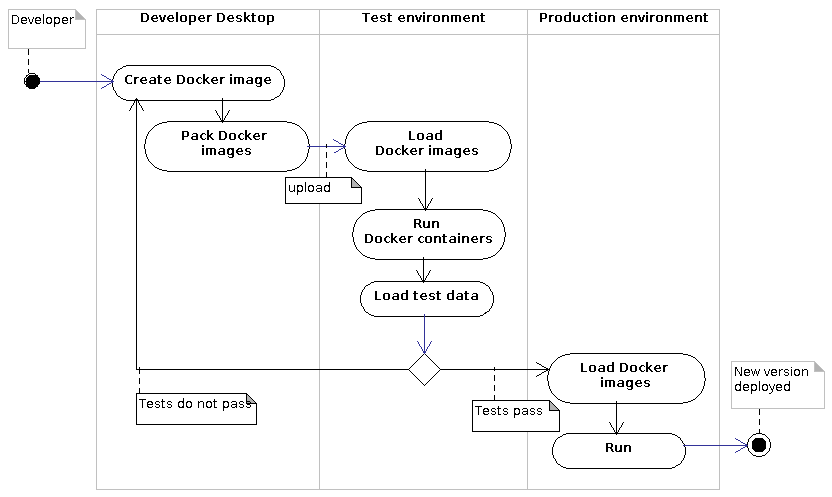
\includegraphics[width=\textwidth]{deploy_wiki_uml.png}
  \end{figure}

\end{frame}

%%%%%%%%%%%%%%
%
% The future
%
%%%%%%%%%%%%%%

% 15. Blick in die Zukunft
\begin{frame}
  \frametitle{Blick in die Zukunft \\ \textcolor{mfn_green}{The shape of things to come}}
  \begin{figure}
    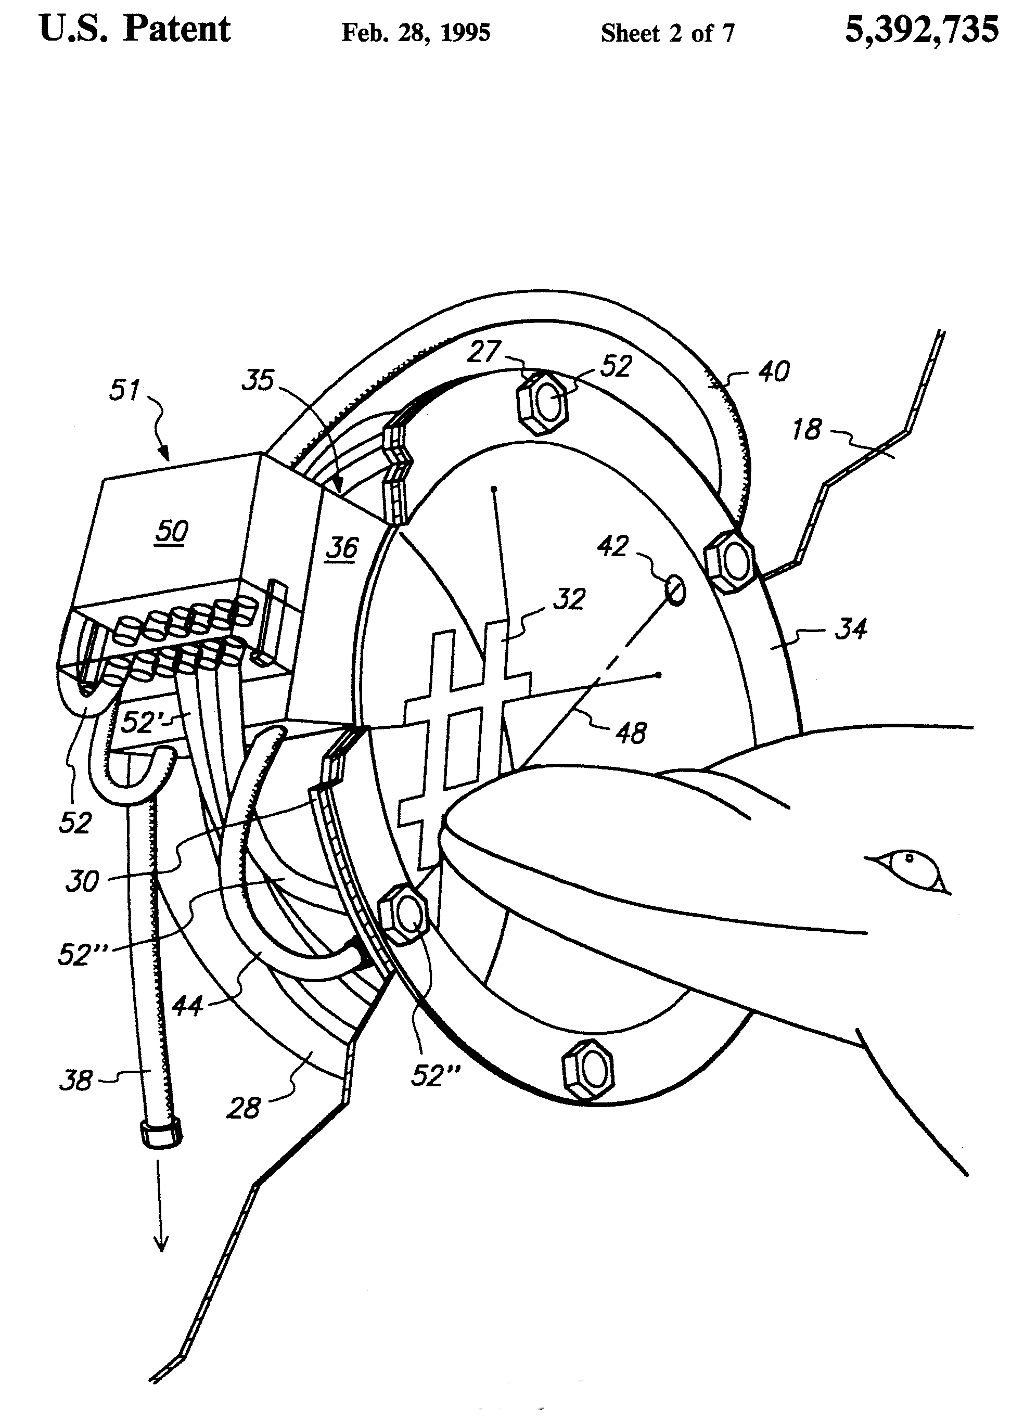
\includegraphics[height=60mm]{marine_mammal_communication.png}
    \caption{Xitco Jr, M.J. et al, 1995. \textit{Marine mammal communication device}. U.S. Patent 5,392,735.}
  \end{figure}
\end{frame}

% 16. Problemzone
% As I'm sure some of you have noticed, the current roll-out process has some disadvantages. One is that the test environment is very prone to failure. As all developers use it, it is often broken and unavailable. Another problem is that much of this stuff is done either by hand or through self-written scripts. This takes time and is not easy to maintain.
\begin{frame}
  \frametitle{Problemzone / \textcolor{mfn_green}{Problem zone}}
  \begin{figure}
    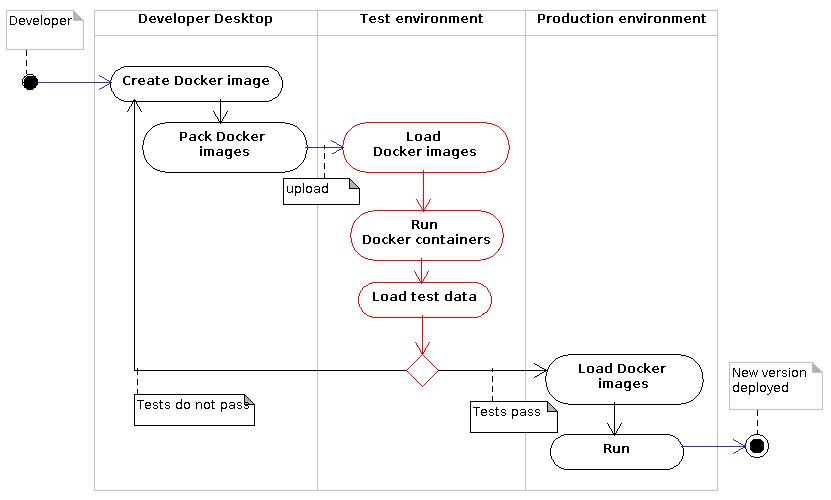
\includegraphics[width=\textwidth]{docker_wikis_problem_uml.png}
  \end{figure}
\end{frame}

% 17. Lösungsansatz
% My current priority is to streamline the roll-out process, by getting rid of the test environment and replacing it with continuous integration. Setting up continuous integration can be a lot of effort, but as anybody who has worked with continuous integration can tell, it is effort well spent. Continuous integration automates the roll-out process, renders testing more transparent, and once it is set up, it is just a mater of submit-and-forget. I am currently planing to use Jenkins to build the continuous integration pipeline. The first step in the pipeline would be to create a disposable virtual machine for testing, using Vagrant. Then the Docker containers would be deployed in the virtual machine, along with some test data. The tests can then run in Selenium. If the tests pass, the result would be deployed to the production environment.
\begin{frame}
  \frametitle{Lösungsansatz / \textcolor{mfn_green}{Planed solution}}
  \begin{figure}
    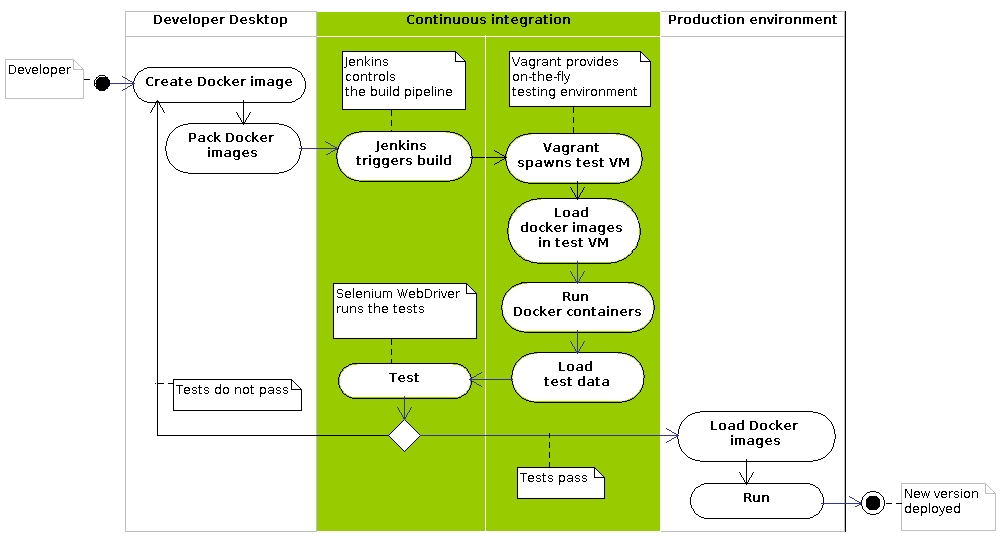
\includegraphics[width=\textwidth]{docker_wikis_integration.png}
  \end{figure}
\end{frame}

% 18. Kontaktdaten
\begin{frame}
  \frametitle{Kontaktdaten / \textcolor{mfn_green}{Contact information}}
  \begin{center}
    Alvaro Ortiz-Troncoso \\
    \medskip
    Email: Alvaro.OrtizTroncoso@mfn.berlin \\    
    \medskip
    Web: https://github.com/MfN-Berlin
  \end{center}
\end{frame}

\end{document}


